% Options for packages loaded elsewhere
\PassOptionsToPackage{unicode}{hyperref}
\PassOptionsToPackage{hyphens}{url}
%
\documentclass[
]{article}
\usepackage{amsmath,amssymb}
\usepackage{lmodern}
\usepackage{iftex}
\ifPDFTeX
  \usepackage[T1]{fontenc}
  \usepackage[utf8]{inputenc}
  \usepackage{textcomp} % provide euro and other symbols
\else % if luatex or xetex
  \usepackage{unicode-math}
  \defaultfontfeatures{Scale=MatchLowercase}
  \defaultfontfeatures[\rmfamily]{Ligatures=TeX,Scale=1}
\fi
% Use upquote if available, for straight quotes in verbatim environments
\IfFileExists{upquote.sty}{\usepackage{upquote}}{}
\IfFileExists{microtype.sty}{% use microtype if available
  \usepackage[]{microtype}
  \UseMicrotypeSet[protrusion]{basicmath} % disable protrusion for tt fonts
}{}
\makeatletter
\@ifundefined{KOMAClassName}{% if non-KOMA class
  \IfFileExists{parskip.sty}{%
    \usepackage{parskip}
  }{% else
    \setlength{\parindent}{0pt}
    \setlength{\parskip}{6pt plus 2pt minus 1pt}}
}{% if KOMA class
  \KOMAoptions{parskip=half}}
\makeatother
\usepackage{xcolor}
\usepackage[margin=1in]{geometry}
\usepackage{color}
\usepackage{fancyvrb}
\newcommand{\VerbBar}{|}
\newcommand{\VERB}{\Verb[commandchars=\\\{\}]}
\DefineVerbatimEnvironment{Highlighting}{Verbatim}{commandchars=\\\{\}}
% Add ',fontsize=\small' for more characters per line
\usepackage{framed}
\definecolor{shadecolor}{RGB}{248,248,248}
\newenvironment{Shaded}{\begin{snugshade}}{\end{snugshade}}
\newcommand{\AlertTok}[1]{\textcolor[rgb]{0.94,0.16,0.16}{#1}}
\newcommand{\AnnotationTok}[1]{\textcolor[rgb]{0.56,0.35,0.01}{\textbf{\textit{#1}}}}
\newcommand{\AttributeTok}[1]{\textcolor[rgb]{0.77,0.63,0.00}{#1}}
\newcommand{\BaseNTok}[1]{\textcolor[rgb]{0.00,0.00,0.81}{#1}}
\newcommand{\BuiltInTok}[1]{#1}
\newcommand{\CharTok}[1]{\textcolor[rgb]{0.31,0.60,0.02}{#1}}
\newcommand{\CommentTok}[1]{\textcolor[rgb]{0.56,0.35,0.01}{\textit{#1}}}
\newcommand{\CommentVarTok}[1]{\textcolor[rgb]{0.56,0.35,0.01}{\textbf{\textit{#1}}}}
\newcommand{\ConstantTok}[1]{\textcolor[rgb]{0.00,0.00,0.00}{#1}}
\newcommand{\ControlFlowTok}[1]{\textcolor[rgb]{0.13,0.29,0.53}{\textbf{#1}}}
\newcommand{\DataTypeTok}[1]{\textcolor[rgb]{0.13,0.29,0.53}{#1}}
\newcommand{\DecValTok}[1]{\textcolor[rgb]{0.00,0.00,0.81}{#1}}
\newcommand{\DocumentationTok}[1]{\textcolor[rgb]{0.56,0.35,0.01}{\textbf{\textit{#1}}}}
\newcommand{\ErrorTok}[1]{\textcolor[rgb]{0.64,0.00,0.00}{\textbf{#1}}}
\newcommand{\ExtensionTok}[1]{#1}
\newcommand{\FloatTok}[1]{\textcolor[rgb]{0.00,0.00,0.81}{#1}}
\newcommand{\FunctionTok}[1]{\textcolor[rgb]{0.00,0.00,0.00}{#1}}
\newcommand{\ImportTok}[1]{#1}
\newcommand{\InformationTok}[1]{\textcolor[rgb]{0.56,0.35,0.01}{\textbf{\textit{#1}}}}
\newcommand{\KeywordTok}[1]{\textcolor[rgb]{0.13,0.29,0.53}{\textbf{#1}}}
\newcommand{\NormalTok}[1]{#1}
\newcommand{\OperatorTok}[1]{\textcolor[rgb]{0.81,0.36,0.00}{\textbf{#1}}}
\newcommand{\OtherTok}[1]{\textcolor[rgb]{0.56,0.35,0.01}{#1}}
\newcommand{\PreprocessorTok}[1]{\textcolor[rgb]{0.56,0.35,0.01}{\textit{#1}}}
\newcommand{\RegionMarkerTok}[1]{#1}
\newcommand{\SpecialCharTok}[1]{\textcolor[rgb]{0.00,0.00,0.00}{#1}}
\newcommand{\SpecialStringTok}[1]{\textcolor[rgb]{0.31,0.60,0.02}{#1}}
\newcommand{\StringTok}[1]{\textcolor[rgb]{0.31,0.60,0.02}{#1}}
\newcommand{\VariableTok}[1]{\textcolor[rgb]{0.00,0.00,0.00}{#1}}
\newcommand{\VerbatimStringTok}[1]{\textcolor[rgb]{0.31,0.60,0.02}{#1}}
\newcommand{\WarningTok}[1]{\textcolor[rgb]{0.56,0.35,0.01}{\textbf{\textit{#1}}}}
\usepackage{longtable,booktabs,array}
\usepackage{calc} % for calculating minipage widths
% Correct order of tables after \paragraph or \subparagraph
\usepackage{etoolbox}
\makeatletter
\patchcmd\longtable{\par}{\if@noskipsec\mbox{}\fi\par}{}{}
\makeatother
% Allow footnotes in longtable head/foot
\IfFileExists{footnotehyper.sty}{\usepackage{footnotehyper}}{\usepackage{footnote}}
\makesavenoteenv{longtable}
\usepackage{graphicx}
\makeatletter
\def\maxwidth{\ifdim\Gin@nat@width>\linewidth\linewidth\else\Gin@nat@width\fi}
\def\maxheight{\ifdim\Gin@nat@height>\textheight\textheight\else\Gin@nat@height\fi}
\makeatother
% Scale images if necessary, so that they will not overflow the page
% margins by default, and it is still possible to overwrite the defaults
% using explicit options in \includegraphics[width, height, ...]{}
\setkeys{Gin}{width=\maxwidth,height=\maxheight,keepaspectratio}
% Set default figure placement to htbp
\makeatletter
\def\fps@figure{htbp}
\makeatother
\setlength{\emergencystretch}{3em} % prevent overfull lines
\providecommand{\tightlist}{%
  \setlength{\itemsep}{0pt}\setlength{\parskip}{0pt}}
\setcounter{secnumdepth}{-\maxdimen} % remove section numbering
\usepackage{booktabs}
\usepackage{longtable}
\usepackage{array}
\usepackage{multirow}
\usepackage{wrapfig}
\usepackage{float}
\usepackage{colortbl}
\usepackage{pdflscape}
\usepackage{tabu}
\usepackage{threeparttable}
\usepackage{threeparttablex}
\usepackage[normalem]{ulem}
\usepackage{makecell}
\usepackage{xcolor}
\ifLuaTeX
  \usepackage{selnolig}  % disable illegal ligatures
\fi
\IfFileExists{bookmark.sty}{\usepackage{bookmark}}{\usepackage{hyperref}}
\IfFileExists{xurl.sty}{\usepackage{xurl}}{} % add URL line breaks if available
\urlstyle{same} % disable monospaced font for URLs
\hypersetup{
  pdftitle={Mixture of contaminated normal distributions with different variables inflation factor within classes},
  pdfauthor={Jorge Sanchez},
  hidelinks,
  pdfcreator={LaTeX via pandoc}}

\title{Mixture of contaminated normal distributions with different
variables inflation factor within classes}
\author{Jorge Sanchez}
\date{2024-02-01}

\begin{document}
\maketitle

\hypertarget{introduction}{%
\subsection{Introduction}\label{introduction}}

The traditional contaminated mixture model assumed that the
contamination is the same for all variables within groups. The
contaminated mixture model each group with a mixture of two normal
distributions with two components. The first normal distribution models
the non-contaminated samples while the second component models the
contaminated samples. The contamination is control by two parameters
which are the proportion of non-contaminated samples in each group
\(\alpha_{g}\) and the inflation factor \(\eta_{g}\) that is the same
for all variables within group.

\[
    f(\mathbf{x}|\vartheta) = \sum^{G}_{g=1} \pi_{g} \left[\alpha_{g} \mathcal{N}(x|\boldsymbol{\mu}_{g},\boldsymbol{\Sigma}_{g})  + (1-\alpha_{g})\mathcal{N}(x|\boldsymbol{\mu}_{g},\eta_{g}\boldsymbol{\Sigma}_{g}) \right]
\] There are cases where the assumption that the inflation factor is the
same for all variables measured in an observation within groups might be
unrealistic. It is possible that the characteristics or variables being
contaminated are a few instead of a all variables. To model this
scenario the previous equation can be modified by replacing the scalar
\(\eta_{g}\) that is the inflation factor for all variables within group
\(g\) by a matrix \(N_{g}\) which is a diagonal matrix where each
element of the diagonal \(\eta_{gj}\) for \(j = 1,\dots,p\) represent
the inflation factor for the corresponding variable.

\[
    f(\mathbf{x}|\vartheta) = \sum^{G}_{g=1} \pi_{g} \left[\alpha_{g} \mathcal{N}(x|\boldsymbol{\mu}_{g},\boldsymbol{\Sigma}_{g})  + (1-\alpha_{g})\mathcal{N}(x|\boldsymbol{\mu}_{g},\dot{N}_{g}\boldsymbol{\Sigma}_{g}\dot{N}^{T}_{g}) \right]
\] \[
\dot{N}_{g} = \begin{bmatrix}
\sqrt{\eta_{g1}} &     0     & \dots     & 0         \\
0         & \sqrt{\eta_{g2}} & \dots     & 0         \\      
\dots     & \dots     & \dots     & \dots     \\
0         &     0     & \dots     & \sqrt{\eta_{gp}} \\   
\end{bmatrix}
\]

\hypertarget{simulation-study-comparison-between-mixtures-with-equal-and-different-inflation-factors-within-group}{%
\subsection{Simulation study: Comparison between mixtures with equal and
different inflation factors within
group}\label{simulation-study-comparison-between-mixtures-with-equal-and-different-inflation-factors-within-group}}

\hypertarget{overview}{%
\subsubsection{Overview}\label{overview}}

In this section, the behavior of contaminated mixture normal models
assuming equal and different variables inflation factor within group is
investigated. To generate the data the following process is conducted to
generate three datasets where \(75\%\) of the samples composed the
training subset and the remaining are part of the test subset.

\begin{enumerate}
\def\labelenumi{\alph{enumi})}
\tightlist
\item
  A contaminated dataset of \(100\) samples in \(p=3\) dimensions and
  same variable inflation factor within group and \(G=1\);
\item
  A contaminated dataset of \(100\) samples in \(p=3\) dimensions with
  different variable inflation factor within group and \(G=1\);
\item
  A contaminated balanced dataset of \(100\) samples in \(p=3\)
  dimensions and \(G=2\) with equal proportions for both groups and one
  group with same variable inflation factor and another group with
  different variable inflation factor;
\end{enumerate}

The parameters for the first dataset are \[
\mu = \begin{pmatrix} 0 \\ 0 \\ 0\\ \end{pmatrix} , \Sigma = I_{3} = \begin{pmatrix} 1 & 0 & 0  \\ 0 & 1 & 0  \\ 0 & 0 & 1   \\ \end{pmatrix}, \alpha = 0.8, \eta = 5
\]

\begin{Shaded}
\begin{Highlighting}[]
\FunctionTok{pairs}\NormalTok{(DatasetA}\SpecialCharTok{$}\NormalTok{Xtrain, }\AttributeTok{col =} \FunctionTok{c}\NormalTok{(}\StringTok{"red"}\NormalTok{,}\StringTok{"blue"}\NormalTok{)[DatasetA}\SpecialCharTok{$}\NormalTok{vtrain }\SpecialCharTok{+} \DecValTok{1}\NormalTok{],}
      \AttributeTok{pch =} \FunctionTok{ifelse}\NormalTok{(DatasetA}\SpecialCharTok{$}\NormalTok{vtrain }\SpecialCharTok{==} \DecValTok{0}\NormalTok{,}\DecValTok{24}\NormalTok{,}\DecValTok{19}\NormalTok{), }\AttributeTok{cex =} \DecValTok{1}\NormalTok{)}
\end{Highlighting}
\end{Shaded}

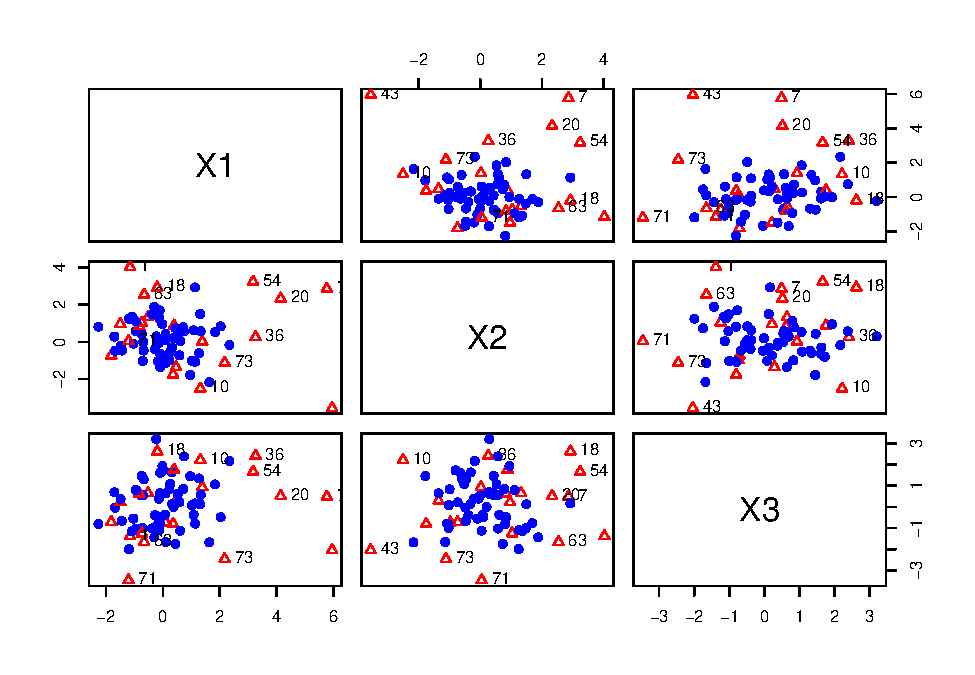
\includegraphics{DifferentVarInflationFactors_files/figure-latex/plotA_training-1.pdf}

Looking at the training data above, it is clear that the inflation
factor is the same across all variables with a few contaminated samples
further than the contaminated samples cloud. This dataset is fitted
firstly with the contaminated mixture of normals model assuming equal
variable inflation factor within group and secondly with the model
assuming different variable inflation factor within group.

The parameter estimates were obtained by using the command Cnmixt until
covergence from the library ContaminatedMixt. Next, the self-coded
E-step was used to obtain the labels whether a sample is
non-contaminated or contaminated. The function Cnmixt assumes equal
variable inflation factor within group and their parameters are shown
below.

\[
\mu = \begin{bmatrix}0.07 \\0.15 \\0.13 \\\end{bmatrix} , \Sigma = \begin{bmatrix}1.05&0&0 \\0&1.05&0 \\0&0&1.05 \\\end{bmatrix}, \alpha = 0.78 , \eta = 4.95
\] The initial values for the parameters of the model were taken from
the contaminated mixture model produced by the function Cnmixt from the
ContaminatedMixt package that assumes same variable inflation factor
within group. Next, an iteration of a self-coded m-step that assumes
different variable inflation factor within group for EII model was run
to obtain the estimated parameters shown below. It is possible to see
that there are some differences between the estimates obtained for both
models. The main difference between the estimates is observed in the
values that the model with different variables inflation factor take for
\(\alpha\) which suggest a \(51\%\) of non-contaminated samples and
implies a greater contamination that the other model. Also, the
inflation factors in the diagonal of the matrix \(\dot{N}\) are
different and much smaller than \(4.95\).

\[
\mu = \begin{bmatrix}0.34 \\0.16 \\0.1 \\\end{bmatrix} , \Sigma = \begin{bmatrix}1.14&0&0 \\0&1.14&0 \\0&0&1.14 \\\end{bmatrix} , \alpha = 0.51, \dot{N} * \dot{N}^{T} = N = \begin{bmatrix}2&0&0 \\0&1.83&0 \\0&0&1.68 \\\end{bmatrix}
\] Next, a self-coded function E-step was used to obtain the estimates
of labels corresponding whether the observations are non-contaminated or
contaminated in the test set. It was observed that the estimates for
\(\alpha\) and \(N\) were affected for the choose of the initial values
of \(\nu_{i}\) which denotes if the \(i^{th}\) sample is
non-contaminated if \(\nu_{i}=1\) otherwise is \(0\). The pairs plot of
the samples in the test subset shows a little more dispersion for the
pair \(X_{1}\) and \(X_{2}\) than for the pair \(X_{1}\) and \(X_{3}\).

\begin{Shaded}
\begin{Highlighting}[]
\FunctionTok{pairs}\NormalTok{(DatasetA}\SpecialCharTok{$}\NormalTok{Xtest, }\AttributeTok{col =} \FunctionTok{c}\NormalTok{(}\StringTok{"red"}\NormalTok{,}\StringTok{"blue"}\NormalTok{)[DatasetA}\SpecialCharTok{$}\NormalTok{vtest }\SpecialCharTok{+} \DecValTok{1}\NormalTok{],}
      \AttributeTok{pch =} \FunctionTok{ifelse}\NormalTok{(DatasetA}\SpecialCharTok{$}\NormalTok{vtest }\SpecialCharTok{==} \DecValTok{0}\NormalTok{,}\DecValTok{24}\NormalTok{,}\DecValTok{19}\NormalTok{), }\AttributeTok{cex =} \DecValTok{1}\NormalTok{)}
\end{Highlighting}
\end{Shaded}

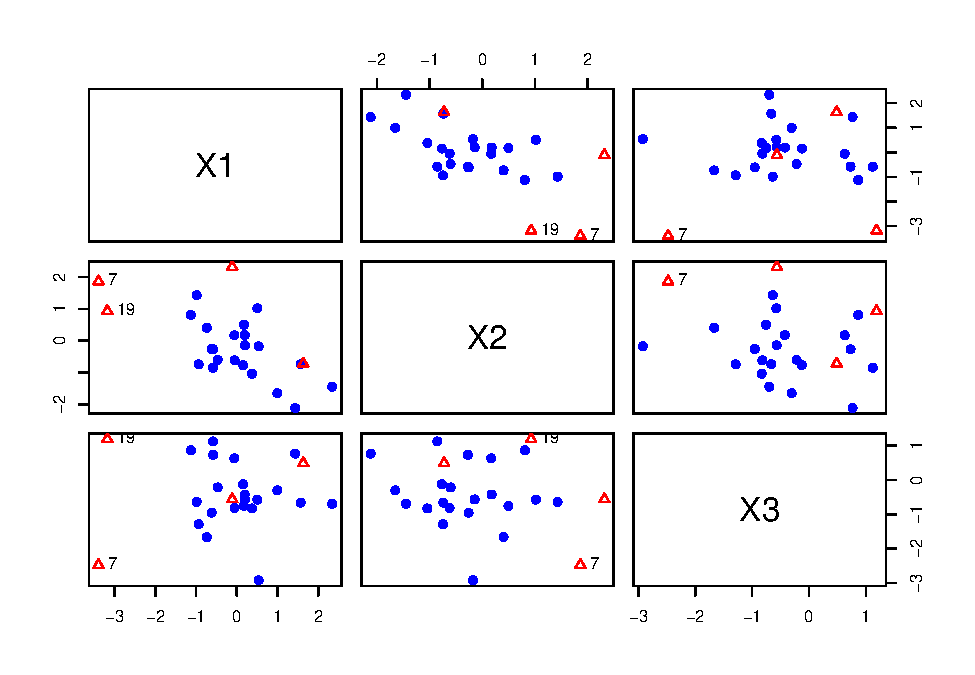
\includegraphics{DifferentVarInflationFactors_files/figure-latex/plotA_test-1.pdf}

The confusion matrix where the rows are the actual values and the
columns the predicted values for the model assuming same variable
inflation factor within group , shows that it was possible to identify
half of the contaminated observations and all the non-contaminated
observations correctly.

\begin{Shaded}
\begin{Highlighting}[]
\NormalTok{knitr}\SpecialCharTok{::}\FunctionTok{kable}\NormalTok{(t\_AEq, }\AttributeTok{format =} \StringTok{"markdown"}\NormalTok{)}
\end{Highlighting}
\end{Shaded}

\begin{longtable}[]{@{}lrr@{}}
\toprule()
& 0 & 1 \\
\midrule()
\endhead
0 & 2 & 2 \\
1 & 0 & 21 \\
\bottomrule()
\end{longtable}

However, taking a look of the performance of the model assuming
different variables inflation factor within group is also able to
identify half of the non-contaminated samples and misclassified \(3\)
non-contaminated samples as contaminated. As the data is generated for a
model with same variable inflation factor within group, there is not
surprise that it overcame their counterpart that assume different
variable inflation factors within group. It is possible to confirm this
result taking a look to the other metrics specially F1\_Score.

\begin{Shaded}
\begin{Highlighting}[]
\NormalTok{knitr}\SpecialCharTok{::}\FunctionTok{kable}\NormalTok{(t\_ADif, }\AttributeTok{format =} \StringTok{"markdown"}\NormalTok{)}
\end{Highlighting}
\end{Shaded}

\begin{longtable}[]{@{}lrr@{}}
\toprule()
& 0 & 1 \\
\midrule()
\endhead
0 & 2 & 2 \\
1 & 3 & 18 \\
\bottomrule()
\end{longtable}

\begin{Shaded}
\begin{Highlighting}[]
\CommentTok{\#knitr::kable(df\_A, format = "markdown")}
\FunctionTok{format\_table}\NormalTok{(df\_A)}
\end{Highlighting}
\end{Shaded}

\begin{verbatim}
##        Metric Equal_IF Different_IF
## 1    Accuracy     0.92         0.80
## 2   Precision     1.00         0.40
## 3      Recall     0.50         0.50
## 4 Sensitivity     0.50         0.50
## 5 Specificity     1.00         0.86
## 6    F1 score     0.67         0.44
\end{verbatim}

The parameters for the second dataset are

\[
\mu = \begin{pmatrix} 0 \\ 0 \\ 0\\  \end{pmatrix} , \Sigma = I_{3} = \begin{pmatrix} 1 & 0 & 0  \\ 0 & 1 & 0  \\ 0 & 0 & 1   \\ \end{pmatrix}, \alpha = 0.8, \dot{N}_{g} = \begin{pmatrix} 1 & 0 & 0 \\ 0 & \sqrt{5} & 0  \\ 0 & 0 & 1  \\  \end{pmatrix}
\] The main different between the second dataset versus the previous one
is that the data is generated from allowing different variables
inflation factor within the group. It is possible to see that \(X_{2}\)
has an inflation factor higher than \(X_{1}\) and \(X_{3}\). The
experiment consist of fitting first the variable assuming the same
variable inflation factor in the group and next allowing different
variable inflation factor within the group and comparing the results
obtained.

\begin{Shaded}
\begin{Highlighting}[]
\FunctionTok{pairs}\NormalTok{(DatasetB}\SpecialCharTok{$}\NormalTok{Xtrain, }\AttributeTok{col =} \FunctionTok{c}\NormalTok{(}\StringTok{"red"}\NormalTok{,}\StringTok{"blue"}\NormalTok{)[DatasetB}\SpecialCharTok{$}\NormalTok{vtrain }\SpecialCharTok{+} \DecValTok{1}\NormalTok{],}
      \AttributeTok{pch =} \FunctionTok{ifelse}\NormalTok{(DatasetB}\SpecialCharTok{$}\NormalTok{vtrain }\SpecialCharTok{==} \DecValTok{0}\NormalTok{,}\DecValTok{24}\NormalTok{,}\DecValTok{19}\NormalTok{), }\AttributeTok{cex =} \DecValTok{1}\NormalTok{)}
\end{Highlighting}
\end{Shaded}

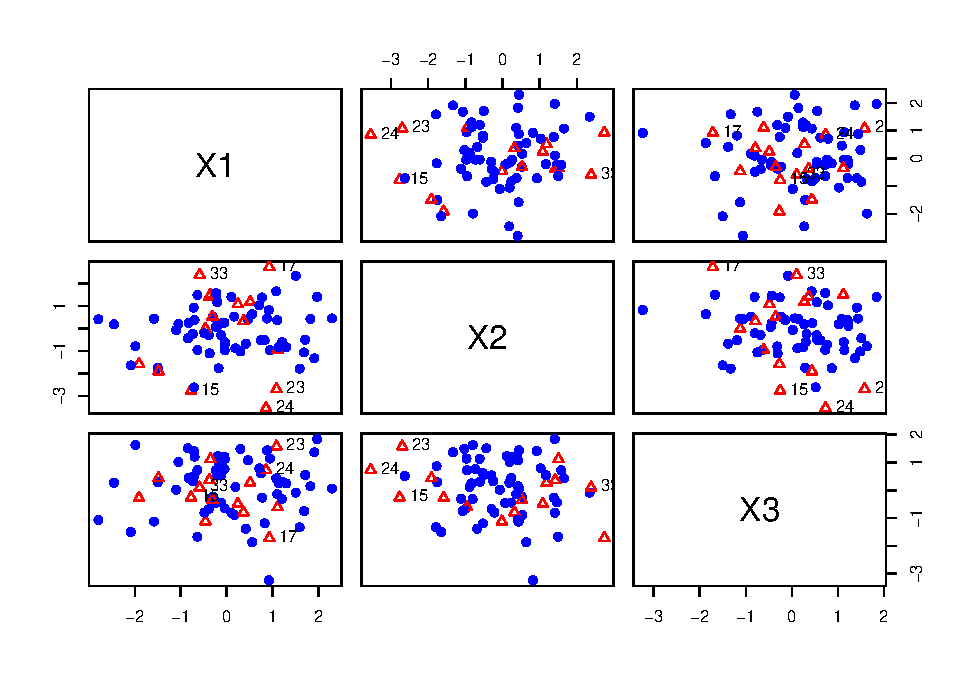
\includegraphics{DifferentVarInflationFactors_files/figure-latex/plotB_training-1.pdf}
It is possible to observed that in the training and test subset there is
a much higher dispersion in the variable \(X2\) in comparison with
\(X_{1}\) and \(X_{3}\).

\begin{Shaded}
\begin{Highlighting}[]
\FunctionTok{pairs}\NormalTok{(DatasetB}\SpecialCharTok{$}\NormalTok{Xtest, }\AttributeTok{col =} \FunctionTok{c}\NormalTok{(}\StringTok{"red"}\NormalTok{,}\StringTok{"blue"}\NormalTok{)[DatasetB}\SpecialCharTok{$}\NormalTok{vtest }\SpecialCharTok{+} \DecValTok{1}\NormalTok{],}
      \AttributeTok{pch =} \FunctionTok{ifelse}\NormalTok{(DatasetB}\SpecialCharTok{$}\NormalTok{vtest }\SpecialCharTok{==} \DecValTok{0}\NormalTok{,}\DecValTok{24}\NormalTok{,}\DecValTok{19}\NormalTok{), }\AttributeTok{cex =} \DecValTok{1}\NormalTok{)}
\end{Highlighting}
\end{Shaded}

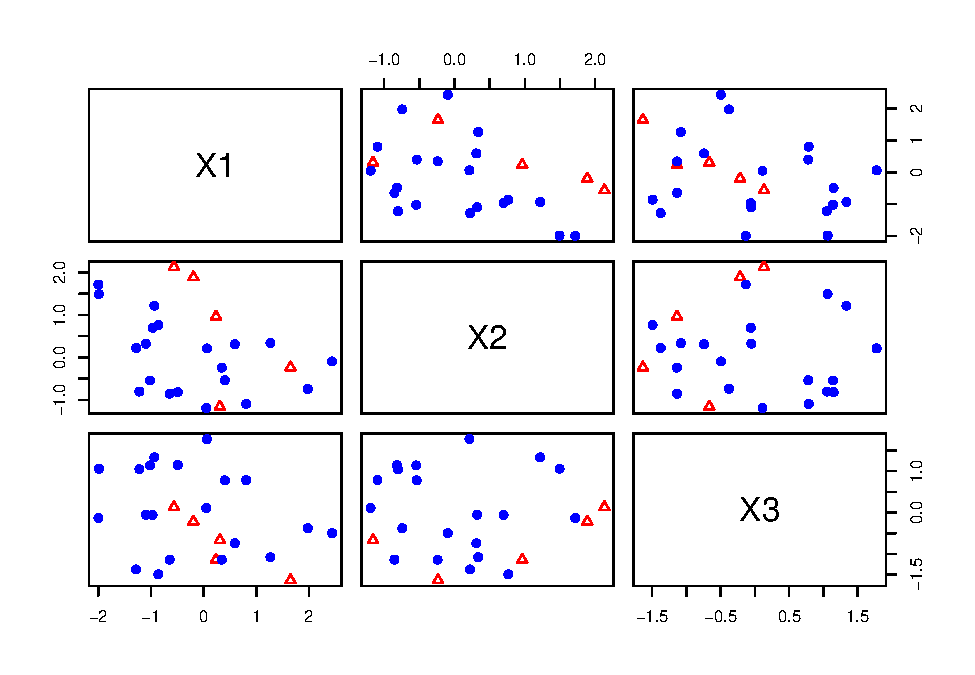
\includegraphics{DifferentVarInflationFactors_files/figure-latex/plotB_test-1.pdf}

Similar procedure is carry out fitting the data with the model EII
assuming same variable inflation factor in the group and the parameters
obtained are:

\[
\mu = \begin{bmatrix}0.06 \\-0.08 \\0.07 \\\end{bmatrix} , \Sigma = \begin{bmatrix}1.22&0&0 \\0&1.22&0 \\0&0&1.22 \\\end{bmatrix}, \alpha = 0.99 , \eta = 1
\]

It is possible to observe that the estimations for \(\mu,\Sigma\) are
quite close, while there is a noticeable different in the estimates for
\(\alpha\) since the estimate parameter assumes there is less
contaminated samples than what the true parameter states. The estimation
for \(\eta\) could be confused by the estimated for \(\lambda\) as the
model fitted is EII. It is possible to see that the value the estimate
takes is \(1.22\) (see diagonal of the variance covariance matrix).

Next, the same data is fit with the model allowing different variables
inflation factor within group and the parameter estimates are shown
below:

\[
\mu = \begin{bmatrix}0.06 \\-0.08 \\0.07 \\\end{bmatrix} , \Sigma = \begin{bmatrix}1.22&0&0 \\0&1.22&0 \\0&0&1.22 \\\end{bmatrix} , \alpha = 0.51, \dot{N} * \dot{N}^{T} = N = \begin{bmatrix}1&0&0 \\0&1.15&0 \\0&0&1 \\\end{bmatrix}
\] The parameters obtained for \(\mu,\Sigma,\) and \(\lambda\) are very
similar as the initial values for the parameters come from the estimates
for the model EII with same variable inflation factor within group. The
main difference between the estimates produced by these two models lies
in the estimates for \(\alpha\) that is \(0.51\) which means that the
inflation factor is being overestimated as the percentage of
non-contaminated samples is \(0.9\). Also, It is possible to see that
the variable inflation factor estimates are different for variables
\(X_{1},X_{2}\) and \(X_{3}\). Also, the estimate for the variable
inflation factor corresponding to \(X_{2}\) is smaller that the true
variable.

Taking a look of the performance of the model assuming same variable
inflation factor within group we can see that it is not able to identify
any of the \(5\) contaminated samples. The plot of the test subset shows
that the contaminated samples are quite close to the non-contaminated
samples.

\begin{Shaded}
\begin{Highlighting}[]
\NormalTok{knitr}\SpecialCharTok{::}\FunctionTok{kable}\NormalTok{(t\_BEq, }\AttributeTok{format =} \StringTok{"markdown"}\NormalTok{)}
\end{Highlighting}
\end{Shaded}

\begin{longtable}[]{@{}lr@{}}
\toprule()
& 1 \\
\midrule()
\endhead
0 & 5 \\
1 & 20 \\
\bottomrule()
\end{longtable}

The model allowing different variables inflation factor within group
performs better than its counterpart that assumes same variable
inflation factor in the group. The former is able to detect \(2\) of the
\(5\) contaminated samples.

\begin{Shaded}
\begin{Highlighting}[]
\NormalTok{knitr}\SpecialCharTok{::}\FunctionTok{kable}\NormalTok{(t\_BDif, }\AttributeTok{format =} \StringTok{"markdown"}\NormalTok{)}
\end{Highlighting}
\end{Shaded}

\begin{longtable}[]{@{}lrr@{}}
\toprule()
& 0 & 1 \\
\midrule()
\endhead
0 & 2 & 3 \\
1 & 2 & 18 \\
\bottomrule()
\end{longtable}

The rest of the metrics confirms that when the data was coming from
different variables inflation factors the model allowing different
inflation factor seems to be more appropiate than assuming equal
inflation factor within group. Nevertheless, more exploration is needed.

\begin{Shaded}
\begin{Highlighting}[]
\CommentTok{\#knitr::kable(df\_A, format = "markdown")}
\FunctionTok{format\_table}\NormalTok{(df\_B)}
\end{Highlighting}
\end{Shaded}

\begin{verbatim}
##        Metric Equal_IF Different_IF
## 1    Accuracy     0.80         0.80
## 2   Precision                  0.50
## 3      Recall                  0.40
## 4 Sensitivity                  0.40
## 5 Specificity     1.00         0.90
## 6    F1 score                  0.44
\end{verbatim}

The parameters for the third dataset are

\[
\mu_{1} = \begin{pmatrix} 0 \\ 0 \\  0 \end{pmatrix} ,  \mu_{2} = \begin{pmatrix} 0 \\ 3 \\ 0 \end{pmatrix}  \Sigma_{1} = I_{3}, \Sigma_{2} = I_{3}, \alpha_{1} = 0.8, \alpha_{2} = 0.9, \eta_{1} = 5,N_{2} = \begin{pmatrix} 1 & 0 & 0  \\ 0 & \sqrt{10} & 0  \\ 0 & 0 & 1  \\\end{pmatrix}
\]

\begin{Shaded}
\begin{Highlighting}[]
\FunctionTok{pairs}\NormalTok{(DatasetC}\SpecialCharTok{$}\NormalTok{Xtrain, }\AttributeTok{col =} \FunctionTok{c}\NormalTok{(}\StringTok{"green"}\NormalTok{,}\StringTok{"blue"}\NormalTok{)[DatasetC}\SpecialCharTok{$}\NormalTok{ltrain],}
      \AttributeTok{pch =} \FunctionTok{ifelse}\NormalTok{(DatasetC}\SpecialCharTok{$}\NormalTok{vtrain }\SpecialCharTok{==} \DecValTok{0}\NormalTok{,}\DecValTok{24}\NormalTok{,}\DecValTok{19}\NormalTok{), }\AttributeTok{cex =} \DecValTok{1}\NormalTok{)}
\end{Highlighting}
\end{Shaded}

\includegraphics{DifferentVarInflationFactors_files/figure-latex/plotC_training-1.pdf}

\begin{Shaded}
\begin{Highlighting}[]
\FunctionTok{pairs}\NormalTok{(DatasetC}\SpecialCharTok{$}\NormalTok{Xtest, }\AttributeTok{col =} \FunctionTok{c}\NormalTok{(}\StringTok{"green"}\NormalTok{,}\StringTok{"blue"}\NormalTok{)[DatasetC}\SpecialCharTok{$}\NormalTok{ltest],}
      \AttributeTok{pch =} \FunctionTok{ifelse}\NormalTok{(DatasetC}\SpecialCharTok{$}\NormalTok{vtest }\SpecialCharTok{==} \DecValTok{0}\NormalTok{,}\DecValTok{24}\NormalTok{,}\DecValTok{19}\NormalTok{), }\AttributeTok{cex =} \DecValTok{1}\NormalTok{)}
\end{Highlighting}
\end{Shaded}

\includegraphics{DifferentVarInflationFactors_files/figure-latex/plotC_test-1.pdf}

\end{document}
